\documentclass[a4paper,12pt]{article}
\usepackage[MeX]{polski}
\usepackage[utf8]{inputenc}
\usepackage{graphicx}

%opening
\title{Raveena Tandon}
\author{Dasher}
\date{31.10.2017}

\begin{document}
\begin{figure}
\maketitle
\end{figure}

\begin{figure}
\section{Najważniejsze informacje}
Raveena Tandon (ur. 1970 w Mumbaju, Indie) --- indyjska, bollywoodzka aktorka i producentka filmowa i modelka. Zadebiutowała w 1991 roku. Została nagrodzona National Film Award.
\end{figure}

\begin{figure}
\section{Wyglad}
\centering
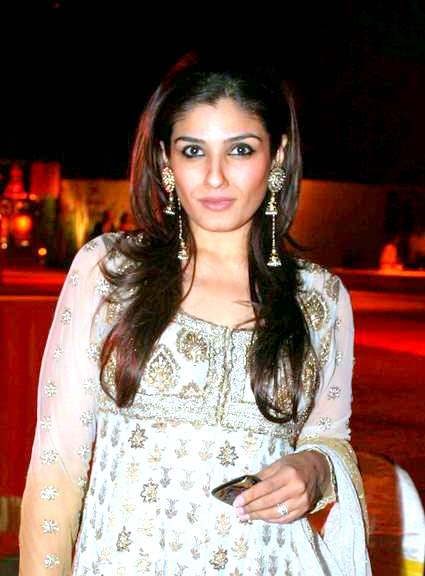
\includegraphics[width=0.25\hsize]{RaveenaTandon.jpg}
\caption{Raveena Tandon}
\end{figure}

\begin{figure}
\section{Filmografia}
\end{figure}
\begin{table}
	\begin{tabular}{c|c|c|c}
	\hline
	\textbf{Rok}&\textbf{Film}&\textbf{Rola}&\textbf{uwagi}\\
	\hline
	1991&Patthar ke Phool&Kiran&Luz New Face Award\\
	\hline
	1992&Parampara&Vijaya\\
	\hline
	&Ek Hi Raasta&Priya Choudhry&\\
	1993&Divya Shakti&Priya\\
	&Pehla Nasha&Neelima&\\
	\hline
	1995&Zamaana Deewana&Priya Malhotra	&\\
	\hline
	&Rakshak&&gościnnie\\
	1996&Ek Anari Do Khiladi&Priya Rao&\\
	&Vijeta&Vijaya&\\
	\end{tabular}
\caption{Filmografia}
\end{table}

\begin{figure}
\tableofcontents
\listoffigures
\listoftables
\end{figure}

\end{document}